\section{Bayesian Optimization}
\label{sec:bayesian-optimization}

This section elaborates upon a method known as \acrfull{acr:bo}, which is used to automate the process of optimizing the parameters of an unknown objective.
First \autoref{sec:bayesian-optimization-problem} introduces the optimization tasks this method is aimed at and how these are relevant to \acrshort{acr:sdm} problems.
Subsequently, in \autoref{sec:bayesian-optimization-algorithm} the optimization method is formally described.
In \autoref{sec:bayesian-optimization-prior-acquisition} the configurable parts of the method are discussed, considering both advantages and disadvantages of available options.
Finally, in \autoref{sec:bayesian-optimization-applications} a number of applications of \acrlong{acr:bo} in the field of planning under uncertainty are discussed, serving as an overview of the method's successes in this field.

% More applications:
%https://www.cs.ox.ac.uk/people/nando.defreitas/publications/BayesOptLoop.pdf

\subsection{Problem Formulation}
\label{sec:bayesian-optimization-problem}

One of the problems that is faced in the field of optimization is that of maximizing a nonlinear, real valued \textit{objective function} $f: \mathcal{X} \mapsto \mathbb{R}$ on a domain $\mathcal{X} \subset \mathbb{R}^m$ ($m \geq 1$).
Formally, to find a global maximizer $x^\ast \in \mathcal{X}$ for which:
\begin{equation}
	x^\ast = \argmax_{x \in \mathcal{X}} f(x)
\end{equation}
In particular the problem turns out to be a common bottleneck when dealing with an objective function that is unknown and expensive to evaluate in terms of the required computational resources.
As an example, one could think of finding the hyper-parameters for a neural network which maximize the performance, where each single evaluation of a set of parameters requires one to train the neural network and assess the performance on a huge dataset.

Although this problem of optimizing expensive functions can be found in many different contexts, it is foremost a problem in \acrshort{acr:sdm}. 
That is, typically one can only hope to estimate objective functions of \acrshort{acr:sdm} problems in AI planning and reinforcement learning through expensive simulations \cite{Brochu2010}. 
A particularly relevant optimization problem pops up when considering the problem of learning to control systems that involve uncertainty, in which an important issue is that of faithfully modeling the uncertainty in the outcomes of actions \cite{Ghahramani2015}.
This particular problem has recently received quite some attention, posing it as a problem of learning and optimizing the parameters of a probabilistic model of the system, such as the model's transition probabilities, reward function or optimal policy \cite{Poupart2010}.

A naive approach for optimizing the objective would be to evaluate a set of (random) combinations of parameters and see which parameter-settings seem to give the best results.
This approach however, usually requires expert knowledge and might demand a large number of function evaluations that do not necessarily provide new information about the parameter-space.
The method known as \textit{\acrlong{acr:bo}}, described in \autoref{sec:bayesian-optimization-algorithm}, improves on these naive approaches by making predictions about which regions of the parameter-space are expected to give the best results and hence limiting the number of function-evaluations.

\subsection{Algorithm Description}
\label{sec:bayesian-optimization-algorithm}

\textit{\acrfull{acr:bo}} is a powerful method for finding the maximum of a typically unknown, expensive, nonlinear objective function, while aiming to minimize the number of objective function evaluations and avoiding local maxima \cite{Brochu2010}.
This method first requires one to set a prior $p(f)$ over the objective function $f$, representing the belief about the space of plausible objective functions.
Then, the algorithm starts off by gathering a small set of initial sample-observation pairs of samples $x \in \mathcal{X}$ and corresponding objective values $y = f(x) + \varepsilon$.
These pairs are then stored in a set $\mathcal{D}_{1:t} = \{(x_i, y_i) \mid i = 1 \ldots t\}$ (i.e., the \textit{evidence set}) where we let $x_i$ denote the $i$th sample and $y_i = f(x_i) + \varepsilon_i$ the corresponding $i$th observation with noise $\varepsilon_i$.
% Posterior / Surrogate Function
The algorithm then derives a posterior distribution $p(f \vert \mathcal{D}_{1:t})$ which, according to Bayes' Theorem, is said to be proportional to the likelihood $p(\mathcal{D}_{1:t} \vert f)$ and the prior $p(f)$ for the first $t$ gathered observations, s.t.:
\begin{equation}
	p(f \vert \mathcal{D}_{1:t}) \propto p(\mathcal{D}_{1:t} \vert f) \cdot p(f)
\end{equation}
This posterior can be viewed as an estimation of the objective function $f$, sometimes referred to as a \textit{surrogate function}.
% It does so by applying Bayes' Theorem, which states that the posterior probability $P(M \vert E)$ of a model $M$ given evidence $E$ is proportional to the likelihood $P(E \vert M)$ of $E$ given $M$

% Acquisition function
To decide on which $x \in \mathcal{X}$ to sample and gather a new observation $f(x)$ from next, a so-called \textit{acquisition function} $a: \mathcal{X} \mapsto \mathbb{R}$ is used, which assigns a certain utility to evaluating $f$ at some particular $x \in \mathcal{X}$ given the evidence set $\mathcal{D}$ at that time.
This acquisition function should be defined such that it captures a correct balance between \textit{exploration} (to sample from areas with high uncertainty) and \textit{exploitation} (to sample from areas likely to improve on prior observations). For this reason many different classes of acquisition functions exist, which are discussed in detail in \autoref{sec:bayesian-optimization-prior-acquisition}.

\begin{figure}
	\centering
	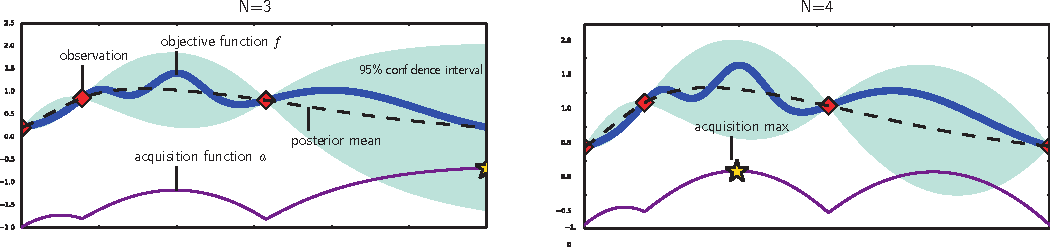
\includegraphics[width=\textwidth]{bo_toy_example_v2}
	\caption{An example of using \acrlong{acr:bo} on a toy example problem. The plots show a \acrshort{acr:gp} approximation of objective function $f$ over four iterations based on $N$ observations. The plots also show the corresponding \acrshort{acr:gp-ucb} acquisition function $a$ for these \acrshort{acr:gp} approximations, which yield high utility for those areas of the domain $\mathcal{X}$ with high prediction uncertainty.}
	\label{fig:bo-toy-example}
\end{figure}

% General Formulation Algorithm

\begin{algorithm}[!t]
	\caption{\acrlong{acr:bo} (General Formulation) \label{alg:bayesian-optimization}}
	\begin{algorithmic}[1]
		\Require{Domain $\mathcal{X} \subset \mathbb{R}^m (m \geq 1)$, prior $p(f)$ and acquisition function $a: \mathcal{X} \mapsto \mathbb{R}$}
		\Let{$\mathcal{D}_{1:n}$}{$\{(x_i, y_i)\}\rvert^{n}_{i=1}$} \Comment{$\mathcal{D}$ is the evidence set with $\mathcal{D}_{1:n}$ the $n$ initial sample-observation pairs}
		\For{$t \gets n + 1, n + 2, \ldots$}
			\Let{$x_t$}{$\argmax_{x \in \mathcal{X}} a(x \vert \mathcal{D}_{1:t-1})$} \Comment{Acquisition based on posterior $p(f \vert \mathcal{D}_{1:t})$}%\Comment{Retrieve the next sample}
			\Let{$y_t$}{$f(x_t) + \varepsilon_t$}  %\Comment{Record a new observation of $f$}
			\Let{$\mathcal{D}_{1:t}$}{$\mathcal{D}_{1:t-1} \cup \{(x_t, y_t)\}$} \Comment{Augment $\mathcal{D}$ with the new evidence}
			\State Update the prior $p(f)$ and posterior $p(f \vert \mathcal{D}_{1:t})$
			\State \textit{Break} when satisfactory \Comment{Stop condition defined by implementation}
		\EndFor
		\State \Return{$\argmax_{(x_i, y_i) \in \mathcal{D}} y_i$}
	\end{algorithmic}
\end{algorithm}

The procedure is illustrated by a toy example in \autoref{fig:bo-toy-example}  with the goal of retrieving the global maximum of the usually unknown objective function $f$.
The prior and acquisition function in this example are set to some of the most common options (i.e., a zero-mean \acrlong{acr:gp} and \acrshort{acr:gp-ucb} function).
The plots show four subsequent iterations which each add a new observation of the objective function $f$ and update the posterior/surrogate function accordingly.
The sample for each next iteration is selected at the point with the highest utility in the acquisition function $a$, in the plots denoted by a star symbol.

The general formulation of the \acrshort{acr:bo} framework is presented in \autoref{alg:bayesian-optimization}.
An implementation of this framework still requires one to define three components, which are the domain $\mathcal{X}$ of $f$, the prior over $f$, and last of all the acquisition function $a$.
The next section discusses the various options that exist for the latter two components in detail.

\newpage

\subsection{Choice of Prior and Acquisition Function}
\label{sec:bayesian-optimization-prior-acquisition}
In order to apply \acrlong{acr:bo} there are two major choices that need to be made, which are those of the prior distribution over the objective and the acquisition function. In this section the different options and corresponding considerations that need to be made for these two components are elaborated upon.

\subsubsection*{Prior Distributions}
\label{sec:bayesian-optimization-prior}
In \acrlong{acr:bo} the \textit{de facto} standard for the prior distribution is a \acrfull{acr:gp}, which is typically well-suited as it accounts for the uncertainty associated with each prediction.
Another important aspect that makes a \acrshort{acr:gp} a convenient choice for the prior distribution is that it induces a posterior distribution over the objective function that is analytically tractable.
Intuitively a \acrshort{acr:gp} can be viewed as a prior which assumes that similar inputs result in similar outputs.
For an objective function $f$, the \acrshort{acr:gp} defines a Gaussian probability distribution over $f(x)$ for each $x$, so that a \acrshort{acr:gp} can be expressed as a probability distribution over functions:
\begin{equation}
	P(f(x) \vert x) = \mathcal{N}(\mu(x), \sigma^2(x))
\end{equation}
where $\mathcal{N}$ denotes a normal distribution, while $\mu$ and $\sigma$ denote mean and standard deviation respectively.
By this definition, a \acrshort{acr:gp} can be viewed as a function that returns the mean and variance of a normal distribution over the possible values of $f$ at $x$. A \acrshort{acr:gp} as prior over an objective function $f$ is typically denoted as: 
\begin{equation}
\label{eq:gp}
f \sim GP(m(\cdot), K(\cdot, \cdot))
\end{equation}
so that the \acrshort{acr:gp} is completely specified by a mean function $m$ and a \textit{kernel} function $K$ defining the covariance.
The mean function $\mu$ is typically initialized by a constant mean, usually zero, due to the assumption that all points in the parameter space are equally likely and because the conditional mean can still be flexibly specified by the kernel function $K$ \cite{kawaguchi2015bayesian}.

The choice of the kernel or covariance function of the \acrshort{acr:gp} determines the smoothness of the estimations on the performance and confidence intervals of unexplored samples in the parameter space.
According to the various literature in the field of \acrlong{acr:bo} the most common kernels are said to be the \textit{squared exponential} (also known as \textit{radial basis function (RBF)} or Gaussian) kernel and Mat\'ern kernel.
However, the squared exponential kernel turns out unrealistically smooth for practical applications \cite{snoek2012practical} and therefore would require properly selecting its hyper-parameters.
The Mat\'ern kernel serves as a more flexible class, where the hyper-parameters allow tweaking the distance at which there are almost no effects from previous samples and the rate at which these effects decrease, for which a reoccurring kernel appears to be an automatic relevance determination (ARD) Mat\'ern 5/2 kernel for machine learning applications \cite{snoek2012practical, kawaguchi2015bayesian}.


%\begin{itemize}
%	\item \acrfull{acr:gp}
%	\item Wiener Process
%\end{itemize}


\subsubsection*{Acquisition Functions}
\label{sec:bayesian-optimization-acquisition}
% Examples acquisition function: PMAX, IEMAX, MPI, MEI, (GP-)UCB, GP-Hedge
% TODO Introduction
The next step is defining an acquisition function which is used in the optimization process to efficiently sample observations towards the global optimum.
Typically, high utility in the acquisition functions corresponds to potentially high objective function values.
However, to avoid getting stuck in local optima, acquisition functions are defined such that a trade-off is made between exploration and exploitation.
In each iteration of the \acrshort{acr:bo} framework, a new observation is sampled at the point $x \in \mathcal{X}$ where the utility is the highest.
Traditionally, the \acrfull{acr:mpi}, \acrfull{acr:mei} and \acrfull{acr:gp-ucb} functions are used for \acrlong{acr:bo} \cite{shahriari2016taking}.
%This section presents an overview of the most common choices for acquisition functions used for Bayesian Optimization, together with their individual advantages and disadvantages.
In the discussion of these acquisition functions, let us define $f(x^+)$ as the `best' observation, corresponding to the sample $x^+ = \argmax_{x_i \in x_{1:t}} y_i$ when considering the first $t$ samples.
In the following overview each of these acquisition functions are defined accompanied by a discussion of their main advantages and disadvantages seen in practice.

% TODO "Best-known acquisition functions:"
\begin{description}
	\item[\acrfull{acr:mpi}] This acquisition function selects the next sample to maximize the probability of improvement, which is the sample $x \in \mathcal{X}$ so that:
	$$\argmax_{x \in \mathcal{X}} P(f(x) \geq f(x^+) + \xi)$$
	where $\xi \geq 0$ is a trade-off parameter. The higher this trade-off parameter $\xi$, the higher the preference of exploration over exploitation. Note that this means that setting $\xi = 0$ implies that the optimization purely depends on exploitation, acquiring points most likely to yield improvement. One could also choose to update $\xi$ dynamically over time.
	\begin{description}
		\item[Advantages] Intuitive acquisition function which can guarantee a minimum improvement of $\xi$ in each iteration. Considers both mean, variance and current best $f(x^+)$ of the surrogate function.
		\item[Disadvantages] Difficult to tune trade-off parameter and extremely sensitive to the choice of this parameter: a too small $\xi$ may result in an exhaustive search around a local optimum, while a too large $\xi$ results in a slow search (close to random sampling)
	\end{description}
	\item[\acrfull{acr:mei}] This acquisition function defines its utility based on the magnitude of the improvement to be expected. The function ignores the points that would lead to a decrease compared to the current best $f(x^+)$. The \acrshort{acr:mei} function selects the point $x \in \mathcal{X}$ such that:
	$$\argmax_{x \in \mathcal{X}} \mathbb{E}[\max(0, \mu_f(x) - f(x^+) - \xi)]$$
	where $\mu_f(x)$ is the posterior mean at $x$ for the objective $f$ and $\xi \geq 0$ a trade-off parameter.
	\begin{description}
		\item[Advantages] Common steps exist for properly setting $\xi$, with $\xi = 0.01$ appearing to work well in most cases according to \cite{lizotte2008practical}. Allows for non-myopic extensions \cite{Brochu2010}.
		\item[Disadvantages] Points that are likely to bring no improvement are neglected, although the chance of them resulting in actual improvement is usually small.
	\end{description}
	\item[\acrfull{acr:gp-ucb}] This acquisition function defines its utility by looking at the curve that is $\beta_t$ standard deviations above the posterior mean $\mu_f$ and samples $x \in \mathcal{X}$ such that:
	$$\argmax_{x \in \mathcal{X}} \mu_f(x) + \beta_t\sigma_f(x)$$
	where $\beta_t$ is an $\mathcal{O}(\log{t})$ exploration coefficient scheduled over time \cite{perchet2014gaussian}. This acquisition function relies on the idea of being optimistic in the face of uncertainty.
	\begin{description}
		\item[Advantages] Strong bounds exist on the cumulative regret and also guidelines exist to set $\beta_t$ to achieve optimal regret.
		\item[Disadvantages] Hyper-parameter $\beta_t$ needs to be set properly.
	\end{description}
\end{description}

In some domains, the time that is needed to evaluate the objective function depends on the region from which a point $x \in \mathcal{X}$ is sampled.
For example, when again the optimization of the hyper-parameters of neural networks is considered, one may observe that for some settings of parameters it takes a lot longer to train a model.
To account for this aspect, one could apply cost-sensitive optimization by using the \acrfull{acr:mei-ps} function.
\begin{description}
	\item[\acrfull{acr:mei-ps}] This acquisition function, proposed in \cite{snoek2012practical}, makes use of another \acrshort{acr:gp}-model over the evaluation time of the objective function over the same domain $\mathcal{X}$.
	The \acrshort{acr:mei-ps} selects the next sample $x \in \mathcal{X}$ such that:
	$$\argmax_{x \in \mathcal{X}} \frac{\mathbb{E}[\max(0, \mu_f(x) - f(x^+) - \xi)]}{\mu_s(x)}$$
	where $\mu_s(x)$ is the posterior mean at $x$ for the timing \acrshort{acr:gp}-model, while $\mu_f$ and $\xi$ are defined as in the \acrshort{acr:mei} function.
	\begin{description}
		\item[Advantages] Prefers samples that are expected to be evaluated with lower cost.
		\item[Disadvantages] Requires another timing \acrshort{acr:gp}-model accompanied by increased costs.
	\end{description}
\end{description}

Further expanding on this, various \textit{portfolio allocation} techniques have been suggested that address the issue that there is no single acquisition function that outperforms the others for all problem instances.
One example is the \textit{\acrshort{acr:gp}-Hedge} algorithm \cite{brochu2010portfolio, shahriari2016taking} which holds a portfolio of acquisition functions and employs past performance of each of these functions to predict their future acquisition performance.
However, this algorithm fails to account for valuable information gained through exploration, which has led to alternative portfolio algorithms, such as the \textit{Entropy Search Portfolio} \cite{shahriari2016taking, wang2016optimization} which considers the gain of information of each acquisition function towards the optimum.

Finally, one can choose to blend the acquisition functions of a set of \acrshortpl{acr:gp} with varying hyper-parameter settings by computing the \textit{integrated acquisition function} \cite{snoek2012practical}:

$$\hat{a}(x\vert\mathcal{D}) = \int a(x\vert\mathcal{D}, \theta_{\mathit{gp}})p(\theta_\mathit{gp}\vert\mathcal{D}) d\theta_{\mathit{gp}}$$

\noindent where $a(x)$ is the utility at $x \in \mathcal{X}$ in the \acrshort{acr:mei} function for the \acrshort{acr:gp} with hyper-parameters $\theta_\mathit{gp}$ given the evidence set $\mathcal{D}$.
Computing $\hat{a}(x)$ is commonly realized by a Monte Carlo integration over the acquisition functions of the \acrshortpl{acr:gp}.
This integrated function is typically used to account for uncertainty in the hyper-parameters of the underlying \acrshort{acr:gp} in the \acrshort{acr:bo} framework.
A benefit of this Bayesian treatment of these hyper-parameters is that the number of choices to be made is reduced and leads to a more automated optimization solution.

%For this acquisition function that is proposed in \cite{snoek2012practical}, another \acrshort{acr:gp}-model is defined over the evaluation time of the objective function for the same domain $\mathcal{X}$.
%So in each iteration the \acrshort{acr:mei-ps} function samples $x \in \mathcal{X}$ such that:

%Apart from the acquisition functions that have been discussed here, there are various other acquisition functions for specific purposes, like for example \textit{Hedge} \cite{hoffman2011portfolio} or \textit{Entropy Search} \cite{wang2016optimization} functions.
%vTODO Discuss shortly and refer to \cite{shahriari2016taking} that these are portfolio acq. functions https://www.cs.ox.ac.uk/people/nando.defreitas/publications/BayesOptLoop.pdf
%TODO Posterior mean or posterior predictive mean?

%Others possible acquisition functions that are used in Bayesian optimization are PMAX, IEMAX and GP-HEDGE. %vTODO

%\subsection{Toy Example}
%\label{sec:bayesian-optimization-toy-example}

\subsection{Applications of Bayesian Optimization to SDM Problems}
\label{sec:bayesian-optimization-applications}

As we consider the optimization of learning probabilistic models for planning under uncertainty in this thesis, it might be valuable to have a look at how \acrlong{acr:bo} is applied to closely related tasks for planning.
Therefore, in this section a number of applications that involve or are closely related to \acrshort{acr:dtp} are highlighted, to get an idea of the applicability of \acrlong{acr:bo} and identify the motivations for using this method.

In \cite{MartinezCantin2009}, \acrlong{acr:bo} is applied for a mobile robot that adaptively plans a path while maximizing the information it obtains from observations about its own location and the location of navigation landmarks in the environment.
The objective/cost function $C$ is parametrized by a policy-vector $\pi$ and approximations for selected samples (of robot pose and landmark locations) are made by different functions over the belief-states of the \acrshort{acr:pomdp} (i.e., average mean square error (AMSE), maximum a posteriori square error (MAPSE) and a largest marginal heuristic).
Typically, estimating the belief-state is an expensive problem, typically carried out through SLAM algorithms in robotics.
Therefore, to minimize computational cost, a \acrlong{acr:bo} algorithm is applied with the choice of a \acrshort{acr:gp}-prior over $C$ and where new samples are acquired using an \acrshort{acr:mei} acquisition function.
Applying \acrlong{acr:bo} allows for a more cost-efficient online path planning method for optimal exploration of an environment compared to other approaches.

Another consideration for exploration of environments with stochastic dynamics is that of safety. That is, the assumption of an \acrshort{acr:mdp} being \textit{ergodic}, which is when any state is reachable from another, is impractical as systems tend to get stuck or break due to unsafe exploration. 
Therefore, in \cite{turchetta2016safe} a method of safe exploration is proposed that, based on an initial set of states that are known a priori to be safe, iteratively identifies which nearby states are safe to visit.
This is done by making regularity assumptions on the safety feature, and by such modeling this safety feature by a \acrshort{acr:gp} prior with a Mat\'ern 5/2 kernel.
The goal of their \texttt{SAFEMDP} algorithm is to visit those states that expand the set of safe states (of which is known that a safe return route exists which is inferred from the \acrshort{acr:mdp}'s transition dynamics) as quickly as possible, so to minimize the resources required to explore the \acrshort{acr:mdp}.
Therefore, the acquisition is performed such that those states are selected that are known to be safe and comprise the highest uncertainty, so that the acquired knowledge with every sample is maximized.

Finally, multiple papers have shown that the \acrshort{acr:bo} framework can be employed to speed up online policy search for \acrshort{acr:rl} tasks.
The proposed algorithms in these papers, have the \acrshort{acr:bo} framework select and evaluate a policy in each iteration and keep track of estimates of the expected value of all policies.
One example is the \texttt{PILCO} framework \cite{deisenroth2011pilco}, a model-based online policy search method, which models the dynamics of a system by a non-parametric \acrshort{acr:gp} so that policies are retrieved indirectly.
Another example is seen in \cite{wilson2014using} in which \acrlong{acr:bo} is used to optimize policies for \acrshort{acr:rl} by exploiting generated trajectory data.
To take advantage of the obtained trajectory information in the \acrlong{acr:bo} this information is intertwined with the kernel of the \acrshort{acr:gp} prior, in such way that the induced behavior (i.e., defined by sequences of selected actions) of pairs of policies are taken into account in a behavior-based kernel (BBK).
Accordingly, given an evidence set $\mathcal{D}_{1:n} = \{(\pi_i, \eta(\pi_i), \xi_i)\}$ an (estimate) of the expected return $\eta(\pi_i)$ of policy $\pi_i$ is computed using a set of trajectories $\xi_i$.
This paper also proposes a model-based \acrlong{acr:bo} method which learns transition probabilities and reward functions based on collected trajectory data to approximate the expected return through simulations on a probabilistic model.
To account for inaccuracies of learned models, this model-based algorithm introduces a $\beta$-term in the kernel that ensures that the model-information is neglected when it turns out to be inaccurate based on the occurrence of systematic errors.

% \cite{martinez2007active}, ... (Robot Planning and Exploration under uncertainty)
